% Drawing 154/08-11 -- folder 154, batch 08, archive page 155 (PDF page 156).
% Transcription: en bas à droite, deux légendes reliées par des accolades au dernier dessin : un fuseau brun autour de la droite verte, la rive supérieure passant par $a$, l'inférieure par $b$ et $c$, avec une flèche vers le haut et une vers le bas ; la première légende est au-dessus du dessin, la seconde au-dessous
% Kind: brown spindle round the green line with banks through a, b, c; legends. Method 2 (schematic redraw from the facsimile). Status: ok.
% Notes: Bottom right: a brown spindle round the green line, the upper bank passing through a, the lower through b and c, an arrow upwards and one downwards; two legends joined to the drawing by braces, one above (« pour d'autres sommets au-dessus » as far as legible; given as text by the transcription) and one below. Read from the page view.
% Coordinates: 1 unit = 1 mm = 1/100 of the crop width (bbox in page fractions: [0.674, 0.403, 0.937, 0.509]).
% Redrawn by Claude (claude-opus-5-5), issue #73, 2026-11-07; not checked by a human; not compiled (no TeX in the session).
% Rights: reproduces part of the work -- behind RENDER_TRANSCRIPTS, never published by itself.
\documentclass[tikz,border=3pt]{standalone}
\usepackage{amsmath,amssymb}
\usetikzlibrary{patterns,arrows.meta}
\tikzset{Or/.style={orange!90!black}, Ye/.style={yellow!80!orange}, Lg/.style={green!60!black!70}, Dg/.style={green!45!black}, Br/.style={brown!80!black}, Rd/.style={red!85!black}, Bl/.style={blue!70!black}, Gy/.style={black!40}, pencil/.style={black!45}, struck/.style={black!35}, mark/.style={circle,draw,inner sep=1.3pt}, pt/.style={circle,fill,inner sep=0.9pt}, opt/.style={circle,draw,fill=white,inner sep=1.1pt}}
\begin{document}
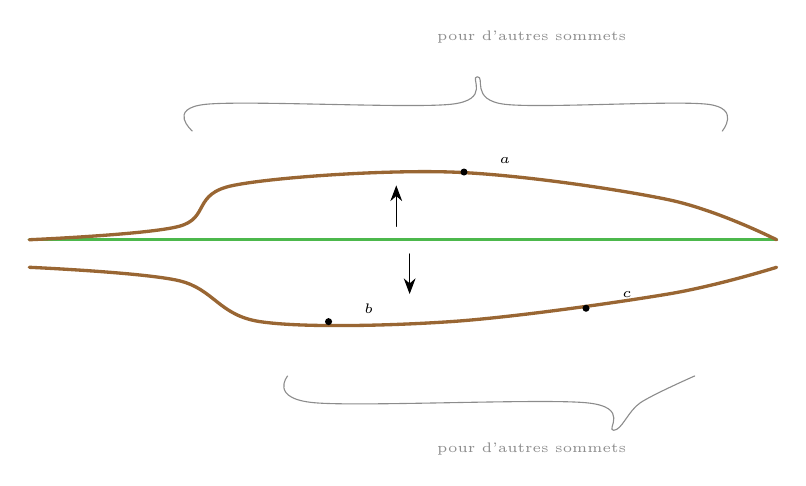
\begin{tikzpicture}[x=1mm,y=1mm,line cap=round,line join=round,font=\scriptsize]
\draw[Lg,very thick] (1.7,-31) -- (96.6,-31);
\draw[Br,very thick] plot[smooth, tension=0.55] coordinates {(1.7,-31) (20.7,-29.3) (27.6,-24.1) (55.2,-22.4) (82.8,-25.9) (96.6,-31)};
\draw[Br,very thick] plot[smooth, tension=0.55] coordinates {(1.7,-34.5) (20.7,-36.2) (31,-41.4) (55.2,-41.4) (82.8,-37.9) (96.6,-34.5)};
\node[pt] at (56.9,-22.4) {};
\node[pt] at (39.7,-41.4) {};
\node[pt] at (72.4,-39.7) {};
\node[inner sep=1pt] at (62.1,-21) {\tiny $a$};
\node[inner sep=1pt] at (44.8,-39.7) {\tiny $b$};
\node[inner sep=1pt] at (77.6,-37.9) {\tiny $c$};
\draw[-{Stealth[length=2mm]}] (48.3,-29.3) -- (48.3,-24.1);
\draw[-{Stealth[length=2mm]}] (50,-32.8) -- (50,-37.9);
\draw[pencil] plot[smooth, tension=0.55] coordinates {(22.4,-17.2) (24.1,-13.8) (55.2,-13.8) (58.6,-10.3) (62.1,-13.8) (87.9,-13.8) (89.7,-17.2)};
\node[inner sep=1pt,pencil] at (65.5,-5.2) {\tiny pour d'autres sommets};
\draw[pencil] plot[smooth, tension=0.55] coordinates {(34.5,-48.3) (37.9,-51.7) (72.4,-51.7) (75.9,-55.2) (79.3,-51.7) (86.2,-48.3)};
\node[inner sep=1pt,pencil] at (65.5,-57.6) {\tiny pour d'autres sommets};
\end{tikzpicture}
\end{document}
